%! alt Acute triangle ABC with BC = 10 along the bottom and A above, near B, with AB + AC = 15. Dashed altitudes from B and C have feet E on CA and F on AB, and segment EF touches the incircle, centred at I. Reflecting EF in the dashed bisector AI gives the segment from E' on AB to F' on AC, which is parallel to BC and touches the incircle at its top, at height twice the inradius above BC.
%! after_paragraph 2
%! scale 4/5
%! let c = (15 - 5*sqrt(6)/3)/2
%! let xa = 5 - 5*sqrt(6)/4
% The shared preamble of every Cevian figure. pipeline/figures turns these colours into theme-aware paint,
% and refuses any other colour, so draw only with them:
%   figink (lines and labels), figaux (construction lines), figaccent (the object the argument turns on),
%   figtint and figaccenttint (light fills).
\documentclass[border=1.5pt]{standalone}
\usepackage{tkz-euclide}
\definecolor{figink}{RGB}{0,0,0}
\definecolor{figaux}{RGB}{85,85,85}
\definecolor{figaccent}{RGB}{192,57,43}
\definecolor{figtint}{RGB}{221,221,221}
\definecolor{figaccenttint}{RGB}{245,213,208}
% tkz-euclide's defaults draw circles, compasses and marks in 50% grey and fill points with a tint.
\makeatletter
\def\tkz@otherlinecolor{figink}
\def\tkz@euc@circlecolor{figink}
\def\tkz@euc@compasscolor{figink}
\def\tkz@euc@mkcolor{figink}
\def\tkz@mk@fill{figink}
\def\tkz@euc@pointfillcolor{figink}
\makeatother
\tkzSetUpLine[color=figink,line width=.7pt]
\tkzSetUpArc[color=figink,line width=.7pt]
\tkzSetUpCompass[color=figink,line width=.5pt]
\tkzSetUpPoint[color=figink,fill=figink,size=3.1pt]
\tikzset{
  every picture/.style={line cap=round,line join=round,color=figink},
  circle style/.append style={color=figink,line width=.7pt},
  aux/.style={color=figaux,line width=.45pt,dash pattern=on 2.6pt off 2pt},
  key/.style={color=figaccent,line width=1pt},
  mk/.style={color=figink,line width=.5pt},
  lbl/.style={color=figink,inner sep=2.2pt},
  len/.style={color=figink,inner sep=1.5pt,font=\small},
}

\begin{document}
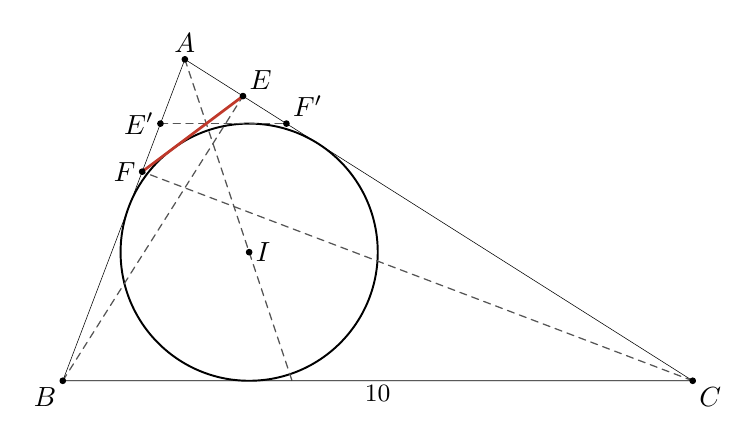
\begin{tikzpicture}
\tkzDefPoint(0.0,0.0){B} %! B = (0, 0)
\tkzDefPoint(8.0000000,0.0){C} %! C = (10, 0)
\tkzDefPoint(1.5505103,4.0824829){A} %! A = (xa, sqrt(c**2 - xa**2))
%! let r = inradius(A, B, C)
\tkzDefPoint(2.2884898,3.6153469){E} %! E = foot(B, C, A)
\tkzDefPoint(1.0084898,2.6553469){F} %! F = foot(C, A, B)
\tkzDefPoint(2.3670068,1.6329932){I} %! I = incentre(A, B, C)
\tkzDefPoint(2.3670068,0.0){D} %! D = foot(I, B, C)
\tkzDefPoint(1.2404082,3.2659863){Ep} %! Ep = reflect(E, A, I)
\tkzDefPoint(2.8404082,3.2659863){Fp} %! Fp = reflect(F, A, I)
\tkzDefPoint(1.3872109,2.9393877){T} %! T = foot(I, E, F)
\tkzDefPoint(2.3670068,3.2659863){U} %! U = foot(I, Ep, Fp)
\tkzDefPoint(2.9113379,0.0){W} %! W = meet(A, I, B, C)
%! fact dist(B, C) == 10
%! fact dist(A, B) + dist(A, C) == 15
%! fact perp(B, E, C, A)
%! fact perp(C, F, A, B)
%! fact tangent(I, r, E, F)
%! fact collinear(Ep, A, B)
%! fact collinear(Fp, A, C)
%! fact parallel(Ep, Fp, B, C)
%! fact tangent(I, r, Ep, Fp)
%! fact dist(A, F) / dist(A, C) == 1/5
%! fact dist(A, E) / dist(A, B) == 1/5
%! fact dist(A, B) * dist(A, C) == 625/12
\tkzDrawCircle(I,D)
\tkzDrawSegments[aux](B,E C,F A,W)
\tkzDrawPolygon(A,B,C)
\tkzDrawSegment[aux](Ep,Fp)
\tkzDrawSegment[key](E,F)
\tkzDrawPoints(A,B,C,E,F,I,Ep,Fp)
\tkzLabelPoint[above,lbl](A){$A$}
\tkzLabelPoint[below left,lbl](B){$B$}
\tkzLabelPoint[below right,lbl](C){$C$}
\tkzLabelPoint[above right,lbl](E){$E$}
\tkzLabelPoint[left,lbl](F){$F$}
\tkzLabelPoint[left,lbl](Ep){$E'$}
\tkzLabelPoint[above right,lbl](Fp){$F'$}
\tkzLabelPoint[right,lbl](I){$I$}
\tkzLabelSegment[below,len](B,C){$10$}
\end{tikzpicture}
\end{document}
